\label{sec:theory}
% Theoretical arguments in the literature closely related to your study

\subsection{Airline business models}
As outlined in the background in section \ref{subsec:b_deregulation} The common trend is that airlines specialize in either of two mayor business models with very different network characteristics.

\subsubsection{Point-to-point network}


\subsubsection{Hub-and-spoke network}
The
A hub-and-spoke network




\begin{figure}[H]
  \centering
  \caption{Point-to-point network (Panel a) vs hub-and-spoke network (Panel b)}
    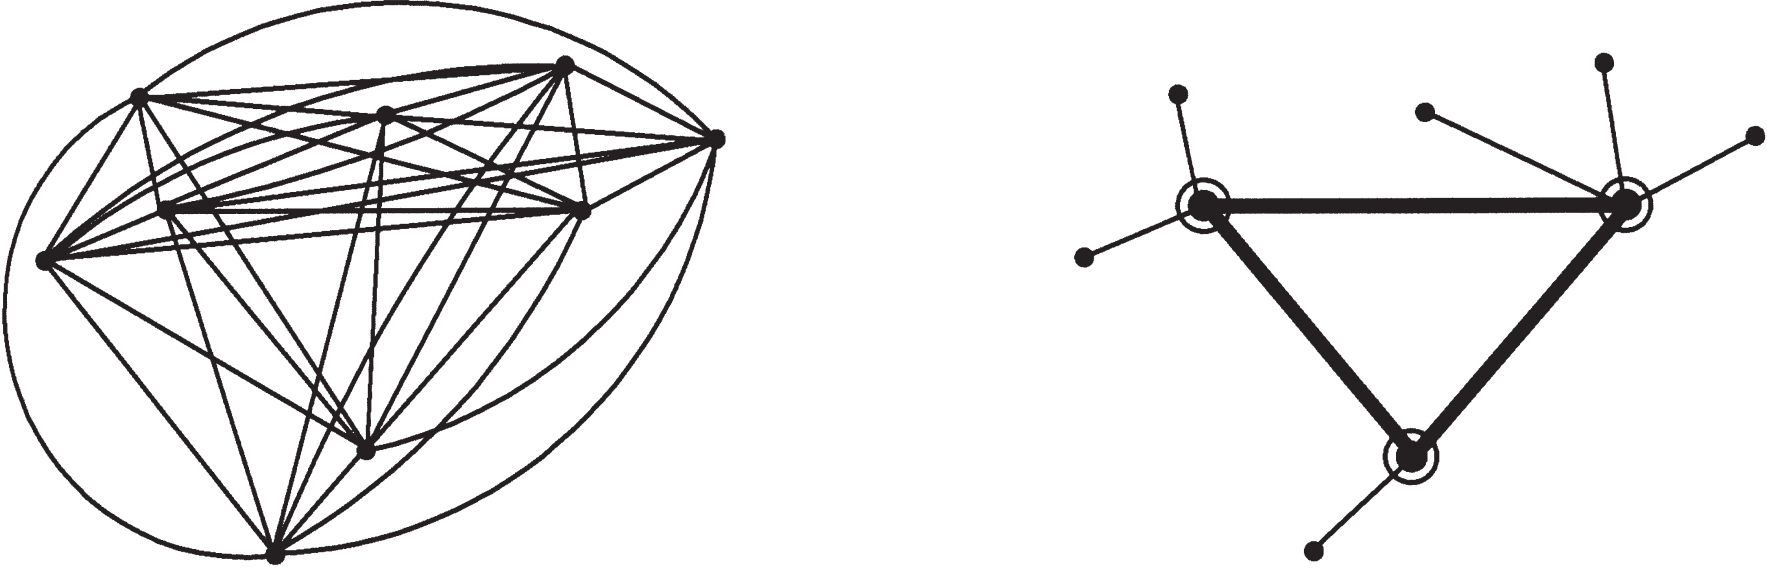
\includegraphics[width=1. \textwidth]{03_figures/Bryan_1999_networks}
    \sourcecenter{\citet{bryan1999hub}}
  \label{fig:Bryan1999}
\end{figure}



\subsection{Network Theory}
\label{subsec:Network Theory}
We draw on network theory to characterize how airports are connected to each other, what role the individual airport plays


%Notes:
